\documentclass[a4paper]{article}
\usepackage[utf8]{inputenc}
\usepackage[french]{babel}
\usepackage[T1]{fontenc}
\usepackage{geometry}
\usepackage{graphicx}

\usepackage{amssymb}
\usepackage{amsmath}
%\usepackage{mathtools}
\usepackage{ifthen}
\usepackage[dvipsnames]{xcolor}

%\usepackage{url}
\usepackage{caption}
\usepackage{subcaption}


\newcommand{\CEDRE}{\emph{CEDRE}}
\newcommand{\PETSc}{\emph{PETSc}}

%\newcommand{\transpose}[2][-3mu]{\ensuremath{\mskip1mu\prescript{\smash{\mathrm t\mkern#1}}{}{\mathstrut#2}}}
\newcommand{\matrixsymb}[2]{\mathcal{M}_{#1}\left(\mathbb{#2}\right)}
%\newcommand{\orthogroup}[2]{\operatorname{O}_{#1}\left(\mathbb{#2}\right)}
\newcommand{\adj}[1]{{#1}^*}
\newcommand{\krylov}[2][]{\ifthenelse{\equal{#1}{}}{\mathcal{K}_{#2}}{\mathcal{K}_{#2}\left({#1}\right)}}
\newcommand{\norm}[2][]{\ifthenelse{\equal{#1}{}}{\left\|{#2}\right\|}{\left\|{#2}\right\|_{{#1}}}}
% \renewcommand{\parallel}{{\mathbin{/\mkern-5mu/}}}


\newcommand{\GP}[1]{\textbf{\color{BurntOrange}{#1}}}
\newcommand{\LM}[1]{\textbf{\color{ForestGreen}{#1}}}
\newcommand{\PS}[1]{\textbf{\color{SkyBlue}{#1}}}


\title{Rapport bibliographique :\\[\baselineskip]\large Méthodologies permettant l’obtention efficace de solutions multi-physiques stationnaires pour des applications en énergétique}
\author{Pierre Seize}
\date{}

\begin{document}
\maketitle

\section{Introduction}

	\subsection{Contexte}

		\paragraph{}
		La nécessité de la simulation numérique est aujourd'hui bien admise, tant dans le monde industriel que le monde académique.
		Les entreprises comme les laboratoires de recherche ont besoin de pouvoir accéder à certaines grandeurs physiques associées à des phénomènes et à des régimes de fonctionnement qui ne sont pas possible de réaliser à notre échelle, la limitation pouvant être matérielle ou bien financière.
		On peut prendre comme exemple l'étude du givrage qui à lieu sur la voilure d'un avion, qui est réalisable expérimentalement mais représente un budget imposant pour l’avionneur, ou bien l'étude des transferts thermiques d'une capsule de rentrée atmosphérique, bien plus difficile à réaliser expérimentalement.
		Pour contourner ces limitations, la simulation numérique est la meilleure option, car elle permet de modéliser un tel cas d'étude par l’exécution d'un programme informatique, et d'obtenir un ensemble important de données qui seront analysées par la suite pour répondre aux questions souhaitées.

		\paragraph{}
		La simulation numérique n'est pas non plus un outil absolu ou parfait : si elle rend possible l'obtention de données inaccessible par l'expérimentation, elle nécessite cependant un travail de modélisation et de développement, des connaissances, et surtout un important travail de calcul informatique.
		Par travail on peut entendre ici une puissance de calcul multiplié par un temps de calcul : n'importe quelle machine ne peut pas réaliser n'importe quelle simulation, certains cas nécessitent des machines très puissantes, et même avec ces machines la simulation numérique n'est pas instantanée, et il est courant de lancer des calculs durant plusieurs semaines.
		Pour éviter de se retrouver avec des calculs qui s'exécuteraient trop longtemps sur des machines trop puissantes, ce qui coûterait trop cher, on va réaliser des choix pour optimiser l'efficacité du calcul.
		On va privilégier un type d'algorithme pour un type de calcul, choisir une mise en donnée plus adaptée qu'une autre pour notre architecture logicielle, ..., tout cela pour réduire le coût en temps et en puissance de calcul de notre simulation numérique.
		C'est pour pouvoir effectuer ces choix qu'il faut posséder des connaissances dans ce domaine.
		L'objectif de ma thèse est d'identifier et de comparer de tels choix qui vont rendre plus efficace la simulation de phénomènes physiques s'inscrivant dans un cadre donné : les problèmes stationnaires en énergétique et multi-physique.

		\paragraph{}
		Il est d'usage de séparer les problèmes de simulation numérique en deux grandes classes : les problèmes instationnaires qui vont décrire l'évolution d'un système au cours du temps, et les problèmes stationnaires qui cherchent la valeur d'un état convergé du même système.
		Cette distinction est déjà bien connue, et engendre déjà des différents choix dans la résolution des problèmes : un problème instationnaire aura un faible pas de temps pour bien capter l'évolution temporelle de chacune des physiques mises en jeu, et utilisera des méthodes d'intégration temporelles explicites, alors qu'un problème stationnaire permet une montée en CFL qui s'accompagne de l'utilisation de méthodes implicites.
		Ma thèse s'intéresse au second type : les problèmes stationnaires.


	\subsection{Le problème stationnaire}

		\paragraph{}
		On considère un problème type de simulation numérique en dynamique des fluides (CFD), qui consiste à résoudre sur un domaine spatial donné une ou un ensemble d'équations décrivant les lois d'évolution du modèle physique.
		Typiquement, on cherche à résoudre une équation aux dérivées partielles :
		$$\frac{\partial W}{\partial t} = \operatorname{f}\left(W\right)$$
		sur un domaine spatial $\mathcal{D}$.
		On note $W$ l'état du système en un point de l'espace.
		Pour un problème stationnaire, l'état du système n'évolue pas, et donc l'équation à résoudre devient :
		\begin{equation}\label{eq:f=0}
			\operatorname{f}\left(W\right) = 0
		\end{equation}
		Concrètement, $W$ représente les grandeurs physiques du système en un point de l'espace et $\operatorname{f}$ une fonction dépendant de l'état du système, mais pouvant également dépendre de ses dérivées spatiales.
		Puisqu'on cherche une solution stationnaire, on l'exprime comme un zéro de cette fonction.
		Pour obtenir cette solution, on introduit la notion de pseudo-temps \cite{KelleyKeyes1996}.
		Par exemple, pour résoudre les équations de Navier-Stokes, les dérivées spatiales d'ordre un et deux interviennent.

		\paragraph{}
		Résoudre l'évolution du système en fonction du temps depuis un état initial connu s'avère souvent plus coûteux que nécessaire, car les états intermédiaires ne nous intéressent pas.
		Inversement, utiliser un algorithme tel que la méthode de Newton de manière brute sur la fonction $\operatorname{f}$ n'aboutit pas.
		Le procédé de plus courant est donc  d'utiliser une méthode introduisant un pseudo-temps (Pseudo-transient continuation method).
		On cherche à résoudre l'équation (\ref{eq:f=0}), et on dispose d'un itéré initial $W_0$.
		On va chercher la solution comme étant la limite en $t = +\infty$ de
		\begin{equation}\label{eq:edp}
			\left\{\begin{aligned}
				\frac{\partial W}{\partial t}\left(t, x\right) = \operatorname{f}\left(W\right) \\
				W\left(t_0, x\right) = W_0\left(x\right)
			\end{aligned}\right.,\qquad \forall x\in\mathcal{D}
		\end{equation}
		La différence avec la résolution d'un problème instationnaire et que les états intermédiaires ne nous intéressent pas, et donc on peut se permettre de calculer des états non physiques, ou des transitions différentes du vrai système physique, du moment que l'état convergé est correct.


	\subsection{Discrétisation}

		\paragraph{}
		Lorsque l'on résout une équation aux dérivées partielles avec une méthode numérique, il est nécessaire de réaliser une discrétisation du problème, ne serait-ce que pour pouvoir représenter l'état du système dans tout le domaine dans un ordinateur.
		En pratique, on réalise deux niveaux de discrétisation : temporel et spatial.

		\paragraph{}
		La discrétisation spatiale consiste à diviser le domaine d'étude $\mathcal{D}$ en un ensemble de cellules qui forment un maillage.
		Les grandeurs physiques étudiées comme la vitesse du fluide, sa température, sa densité, ..., sont alors représentés dans chaque cellules, par leur valeur moyenne, ou leur valeur sur chaque interface, ou de manière plus complexe en fonction du choix de discrétisation pris par l'utilisateur.
		Sans rentrer dans les détails, puisque cette problématique de discrétisation spatiale ne rentre pas dans le cadre de ma thèse, l'état physique dans l'ensemble du domaine est représenté non plus par une fonction $W : \mathcal{D} \rightarrow \mathbb{R}^n$ mais par un vecteur $W \in \mathbb{R}^{N\times n}$, en notant $n$ le nombre de degrés de liberté et $N$ le nombre de cellules du maillage.
		La discrétisation spatiale donne également un moyen de calculer les dérivées spatiales de l'état en fonction de l'état.
		Ainsi l'équation aux dérivées partielles (\ref{eq:edp}) peut se réécrire comme une équation différentielle ordinaire :
		\begin{equation}\label{eq:edo}
			\left\{\begin{aligned}
				\frac{\mathrm{d} W}{\mathrm{d} t}\left(t\right) = f\left(W\right) \\
				W_0 \in \mathbb{R}^{N\times n}
			\end{aligned}\right.
		\end{equation}
		Puisque ma thèse ne s'intéresse pas à la discrétisation spatiale, nous nous placerons dans le cas général et chercherons à résoudre l'équation (\ref{eq:edo}).


		\paragraph{}
		La discrétisation temporelle permet de représenter le temps continu par une succession de temps discrets.
		On va donc représenter et calculer la solution non pas sur l'ensemble du temps mais en ces instants discrets.
		Concrètement, à l'instant $t_n$ on transforme l'équation aux dérivées partielles en relation de récurrence, entre l'état suivant à calculer $W_{n+1}$, l'état actuel $W_n$ et d'éventuels états précédents $W_i$.

		\paragraph{}
		Si on peut exprimer l'état suivant $W_{n+1}$ directement à partir de l'état courant (et éventuellement des précédents), la méthode d'intégration temporelle est dite explicite.
		L'intérêt d'une telle méthode est qu'elle permet de calculer l'état suivant très rapidement, souvent par la simple évaluation d'une fonction.
		Cependant, ces méthodes ont tendance à devenir instable dès que le nombre de Courant devient un peu grand (typiquement 1) et imposent donc l'utilisation de très faibles pas de temps.
		Puisque l'on cherche la solution au bout d'un temps long pour le problème stationnaire, l'utilisation de ces méthodes ne s'avère pas rentable : il vaut mieux payer plus cher l'itération mais converger plus rapidement, et c'est pour cela qu'on utilise les méthodes implicites.
		Elles se caractérisent par le fait que l'état suivant ne s'exprime pas explicitement à partir des états connus, mais qu'il est solution d'une équation, par exemple le zéro d'une fonction.



\section{Résolution implicite d'une Équation aux Dérivées Partielles}

	\subsection{Étapes}

		\paragraph{}
		Nous cherchons à résoudre l'équation (\ref{eq:edo}) en utilisant une méthode d'intégration implicite.
		Pour comprendre le fonctionnement des méthodes d'intégration temporelles implicites, on peut regarder la plus simple : la méthode d'Euler implicite.
		Elle consiste à intégrer entre $t_n$ et $t_{n+1}$ l'équation en gardant un second membre constant à $t = t_{n+1}$.
		Alors, en notant $\Delta t = t_{n+1} - t_n$ et $\Delta W = W_{n+1} - W_n$:
		$$\Delta W = \Delta t f\left(W_{n+1}\right)$$
		On voit que l'incrément de l'état $\Delta W$ peut s'exprimer comme le zéro d'une fonction : on cherche le zéro de $\delta W \mapsto \delta W - \Delta t f\left(W_n + \delta W\right)$.
		En notant $\operatorname{F}$ cette fonction, on obtient l'équation non-linéaire :
		\begin{equation}\label{eq:non_linear}
			\operatorname{F}\left(\delta W\right) = 0
		\end{equation}
		Nous allons donc devoir résoudre une équation non-linéaire à chaque itération.

		\paragraph{}
		Pour résoudre l'équation (\ref{eq:non_linear}), on utilise par exemple la méthode de Newton.
		On part d'une valeur initiale de l'incrément $\delta W_0 = 0$, mais on peut envisager de prendre d'autres valeurs, comme $\Delta t f\left(W_n\right)$ qui est l'incrément donné par la méthode d'Euler explicite.
		On va ensuite itérer pour trouver le zéro de $\operatorname{F}$.
		La linéarisation à l'ordre 1 de l'équation (\ref{eq:non_linear}) s'écrit :
		$$F(\delta W) = -\Delta t f\left(W_n\right) + \left(\mathrm{I} - \Delta t J_n\right)\delta W = 0$$
		où $J_n$ est la matrice jacobienne de $f$, et on exprime donc l'incrément comme étant la solution d'un système linéaire :
		\begin{equation}\label{eq:linear}
			A\delta W = b
		\end{equation}
		avec la matrice $A = \mathrm{I} - \Delta t J_n$ et le second membre $b = \Delta t f\left(W_n\right)$.
		A chaque étape de l'algorithme de Newton, il faut résoudre un système linéaire.

		\paragraph{}
		Pour toutes les méthodes d'intégration temporelles implicites, on retrouve la même idée : pour chaque itération on résout une équation non-linéaire (\ref{eq:non_linear}), en résolvant un ou plusieurs systèmes linéaires (\ref{eq:linear}).
		Les performances d'un code de calcul sont donc très étroitement liées à sa capacité à résoudre efficacement ces systèmes linéaires.



\section{Résolution du système linéaire}

	\paragraph{}
	On s'intéresse ici à la résolution numérique d'un système linéaire $Ax = b$, de taille $N$, c'est à dire que l'on cherche $x\in\mathbb{K}^N$ avec le second membre $b\in\mathbb{K}^N$ et la matrice $A\in\matrixsymb{N}{K}$ connus.
	Dans le cadre de l'énergétique et de la multi-physique, les équations sont réelles mais pour plus de généralité on prend le corps $\mathbb{K} = \mathbb{R}\textrm{ ou }\mathbb{C}$.


	\subsection{Système linéaire creux}

		\paragraph{}
		Comme cela a été mentionné, la taille des matrices rencontrées dans un problème typique de la simulation numérique de la dynamique des fluides est très grande.
		Les matrices ont également une autre propriété : la creusité.
		Puisque les matrices des systèmes linéaires à résoudre sont liées à une matrice jacobienne (voir équation (\ref{eq:linear})), un coefficient de la matrice symbolise une interaction entre deux points du maillage.
		On comprend alors que si le graphe de ces interactions dépend du schéma de discrétisation et d'intégration spatiale, deux points éloignés dans le maillage ne seront pas reliés.
		Ainsi, les matrices présentent cette caractéristique notable qu'est la creusité et que l'on peut observer sur la figure \ref{fig:sparse}.
		On y voit en effet que la majorité des coefficients du système linéaire sont 0.
		En pratique, les matrices rencontrées sont tellement grandes qu'il n'est pas possible de les stocker et de les utiliser sous leur forme dense.
		La propriété de creusité permettra d'utiliser des représentation astucieuses pour stocker les matrices en mémoire, telle que le format CSR (Compressed Sparse Row) \cite{Saad2003}.
		Ces formats permettent à la fois d'économiser de l'espace en mémoire lors du stockage de la matrice, mais également de réaliser des opérations telles que le produit matrice vecteur plus efficacement qu'avec une matrice dense de même taille.

		\begin{figure}
			\centering
			\begin{subfigure}[t]{0.3\textwidth}
				\centering
				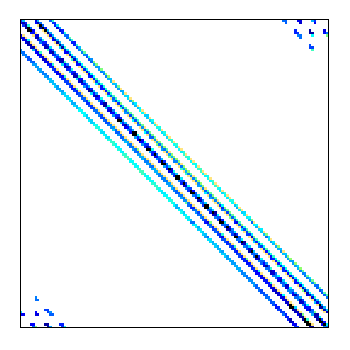
\includegraphics[width=\textwidth]{images/GT01R.png}
				\caption{GT01R : écoulement 2D non visqueux à travers un étage d'aubes de turbomachine}
				\label{fig:sparse.GT01R}
			\end{subfigure}
			\hfill
			\begin{subfigure}[t]{0.3\textwidth}
				\centering
				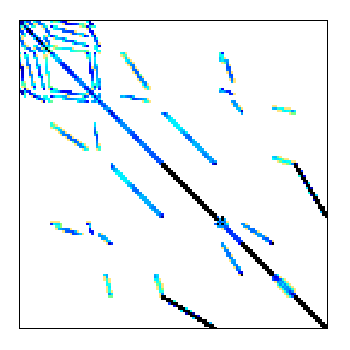
\includegraphics[width=\textwidth]{images/HV15R.png}
				\caption{HV15R : écoulement RANS 3D dans la soufflante d'un moteur}
				\label{fig:sparse.HV15R}
			\end{subfigure}
			\hfill
			\begin{subfigure}[t]{0.3\textwidth}
				\centering
				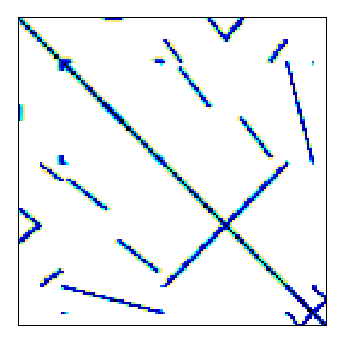
\includegraphics[width=\textwidth]{images/RM07R.png}
				\caption{RM07R : écoulement 3D visqueux dans le compresseur d'un turbopropulseur}
				\label{fig:sparse.RM07R}
			\end{subfigure}
			\caption{Représentation de matrices issues de problèmes de CFD \cite{PacullAubertBuisson2011}, utilisant une méthode spatiale Volumes Finis, les points de couleurs correspondant aux valeurs non nulles}
			\label{fig:sparse}
		\end{figure}


	\subsection{Type de méthode}
		\paragraph{}
		Il existe un grand nombre de méthodes pour inverser un problème linéaire.
		Cependant, en simulation numérique de la dynamique des fluides, la taille des maillage est souvent très importante (\PS{PAR EXEMPLE ?}), ce qui engendre des systèmes de très grande taille.
		Certaines méthodes de résolution ne sont alors plus compatibles, comme en particulier les méthodes directes.
		Cette famille de méthodes, dont fait partie par exemple la méthode du pivot de Gauss, calcule exactement la solution du système linéaire, mais nécessite un temps de calcul très important et un espace mémoire déraisonnable pour les tailles de nos problèmes.
		À l'inverse, les méthodes itératives produisent une suite de vecteurs qui convergent vers la solution du système linéaire.
		L'erreur sur la résolution du système décroît à mesure que l'algorithme itère et cela permet d'atteindre la précision souhaitée, non nulle mais suffisamment petite, pour un temps de calcul et une consommation mémoire maîtrisé.
		C'est l'idée que l'on retrouve sur la figure \ref{fig:direct-iterative} : la méthode directe ne fait aucun progrès avant $O\left(N^3\right)$ opérations, alors que la norme de l'erreur décroît pour la méthode itérative.

		\begin{figure}
			\centering
			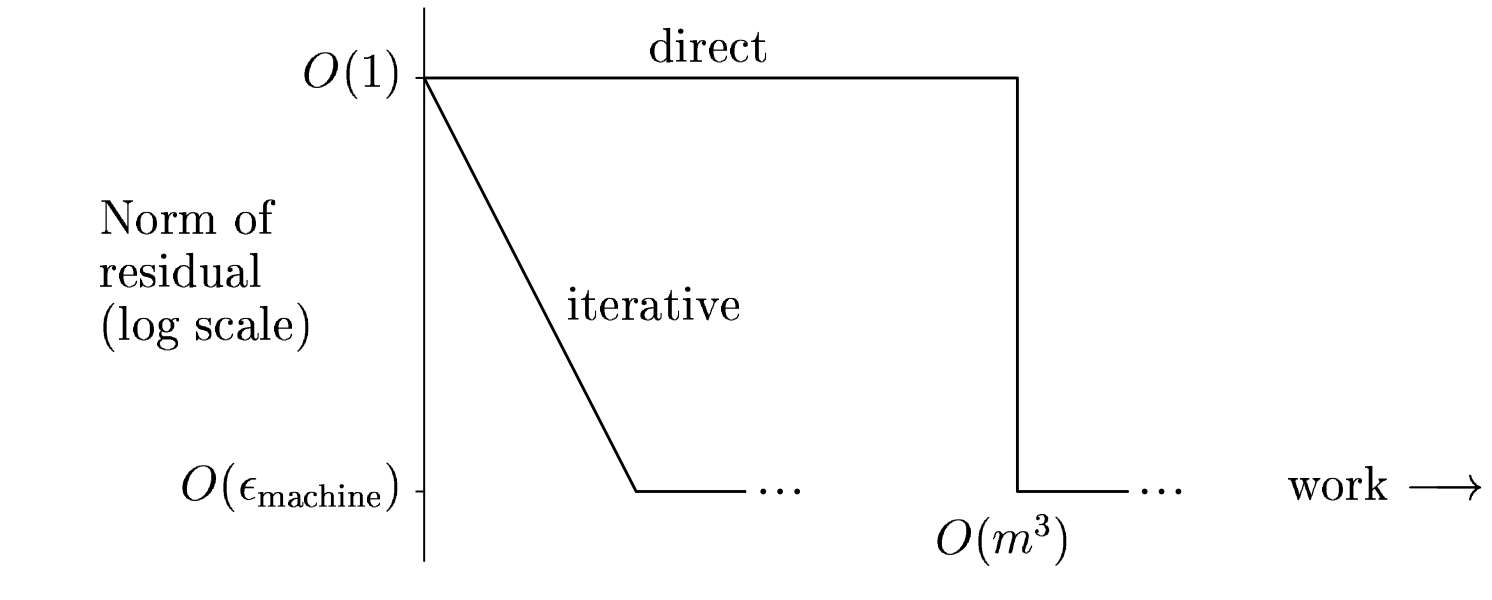
\includegraphics[width=.7\textwidth]{images/direct-iterative.png}
			\caption{Convergence des méthodes directes et itératives, issu de \cite{TrefethenBau1997}}
			\label{fig:direct-iterative}
		\end{figure}

		\paragraph{}
		Les méthodes itératives sont donc les plus adaptées pour inverser des systèmes linéaires creux de grande taille.
		Cependant, il peut arriver qu'on utilise une méthode directe : on peut envisager par exemple la résolution d'un système linéaire avec une succession d'étages d'un algorithme multigrille, pour arriver à un système grossier de petite taille (ou du moins de taille raisonnable), qu'on résoudrait avec une méthode directe comme la décomposition LU.
		Ces méthodes sont bien connues \cite{TrefethenBau1997}, et ne seront pas détaillées ici.


	\subsection{Méthodes itératives}

		\paragraph{}
		Les méthodes itératives sont encore aujourd'hui très étudiées dans la communauté des mathématiques appliquées \cite{OlshanskiiTyrtyshnikov2014, Saad2003, TrefethenBau1997}.
		Une première classe de méthode intervient : les méthodes itératives classiques.
		Si ces méthodes sont plutôt anciennes et plutôt écartées pour leurs mauvaises performances, elles peuvent s'utiliser en se combinant avec des méthodes plus efficaces, et c'est pour cela qu'il est important de comprendre leur fonctionnement.
		Ce sont des méthodes de relaxation, parmi lesquelles on compte les méthode de Jacobi, Gauss-Seidel ou encore SOR (successive over relaxation).
		Leur fonctionnement réside dans une décomposition $A = M - N$ avec $M$ une matrice facile à inverser, où le choix des matrices est propre à la méthode.
		Pour la méthode de Jacobi on prendra pour $M$ la diagonale de $A$.
		Il suffit ensuite, à partir d'un itéré initial $x_0$ d'appliquer la formule de récurrence $x_{k+1} = M^{-1}\left(Nx_k + b\right)$.
		Cependant, comme dit précédemment, ces méthodes n'offrent pas une convergence satisfaisante pour la communauté de CFD.
		Ainsi, il faut se tourner vers un autre type de méthodes itératives pour résoudre le système linéaire.

	\subsection{Méthodes de Krylov}

		\paragraph{}
		Les méthodes de Krylov apparaissent comme étant la norme dans le domaine de la dynamique des fluides numérique.
		Le principe d'une méthode de Krylov est de projeter le système linéaire sur un espace restreint appelé espace de Krylov, et d'y résoudre le système maintenant qu'il est plus petit.
		L'astuce va être dans le fait que ces espaces de Krylov sont emboîtés, et qu'a chaque nouvelle itération on utilise l'information accumulée lors des précédentes.

		\paragraph{}
		Dans ce qui suit, on notera à l'itération $n$ le résidu $r_n = b - Ax_n$, où $x_n$ est l'itéré produit par l'algorithme à l'itération $n$.
		Dans la pratique, on se restreint à un nombre d'itérations $n\ll N$ pour des raisons évoquées précédemment, mais la suite reste vraie pour $n\le N$.
		On supposera également que l'équation (\ref{eq:linear}) admet une solution.
		Enfin, on notera que résoudre $Ax = b$ avec un itéré initial $x_0$ est équivalent ici à résoudre $A\tilde{x} = b - Ax_0$ avec un itéré initial nul, puis prendre $x_0 + \tilde{x}$ comme vecteur solution.

		\paragraph{}
		Pour résoudre $Ax = b$ en partant d'un itéré initial $x_0$ et donc d'un résidu $r_0 = b - Ax_0$, on définit l'espace de Krylov à l'itération $n$:
		\begin{equation}\label{eqn:krylov}
			\krylov[A, r_0]{n} = \operatorname{Vect}\left(r_0, Ar_0, \dots, A^{n-1}r_0\right)
		\end{equation}
		On constate alors que $\krylov{1}\subset\krylov{2}\subset\dots\subset\krylov{n-1}\subset\krylov{n}$.
		On cherche ensuite l'itéré sur $\krylov{n}$ qui garantit une condition de Petrov-Galerkin \cite{SimonciniSzyld2007} :
		\begin{equation}\label{eqn:x_n}
			x_n \in x_0 + \krylov[A, r_0]{n}\quad\textrm{tel que}\quad x_n \perp \mathcal{L}_n
		\end{equation}
		où $\mathcal{L}_n$ est un sous-espace vectoriel de dimension $n$.
		Pour $\mathcal{L}_n = \krylov{n}$ on parle de condition de Galerkin, et pour $\mathcal{L}_n = A\krylov{n}$ de minimisation du résidu.
		On voit donc que si $A$ est inversible, alors l'algorithme termine en au plus $N$ itérations.
		n+1Cette remarque reste informative puisqu'en pratique on arrêtera l'algorithme bien avant.

		\paragraph{}
		Pour construire les différents espaces de Krylov, on utilise l'itération d'Arnoldi \cite{TrefethenBau1997}.
		La matrice $A$ est semblable à une matrice de Hessenberg $H$ :
		\begin{equation}\label{eq:hessenberg}
			A = \adj{V}HV\quad\textrm{avec}\quad H=
			\begin{pmatrix}
				h_{1,1}&h_{1,2}&h_{1,3}&\cdots &h_{1,N}\\
				h_{2,1}&h_{2,2}&h_{2,3}&\cdots &h_{2,N}\\
				0      &h_{3,2}&h_{3,3}&\cdots &h_{3,N}\\
				\vdots &\ddots &\ddots &\ddots &\vdots \\
				0      &\cdots &0      &h_{N,N-1}&h_{N,N}
			\end{pmatrix}
		\end{equation}
		Dans (\ref{eq:hessenberg}), $V$ est une matrice orthonormale de taille $N$.
		On notera $v_i$ sa $i^{\textrm{ème}}$ colonne.
		On notera également $V_n\in\matrixsymb{N, n}{K}$ la matrice constituée des $n$ premières colonnes de $V$.
		On notera enfin $\widetilde{H}_n\in\matrixsymb{n+1, n}{K}$ le bloc supérieur gauche de $H$, qui est également de Hessenberg.

		\paragraph{}
		En considérant les $n \le N$ premières colonnes de (\ref{eq:hessenberg}), on obtient l'équation


		\paragraph{}
		Il existe donc beaucoup de méthodes de Krylov pour résoudre un système linéaire, la distinction entre elle se faisant par le choix à chaque itération du sous-espace $\mathcal{L}_n$.
		La condition de minimisation du résidu donne la méthode GMRES, qui est l'une des plus utilisée par les communautés de CFD et de mathématiques appliquées.
		Elle permet, après des itérations un peu plus coûteuses que ses consœurs telles que la méthode Bi-CG \cite{TrefethenBau1997}, de minimiser le résidu obtenu et donc de garantir une décroissance de l'erreur.
		De plus, la méthode GMRES est beaucoup étudiée et de nombreuses variantes et améliorations ont été développées au fil des années.
		Pour ces raisons, et parce que son implémentation est relativement simple, c'est sur cette méthode que j'ai décidé de m'orienter.


	\subsection{GMRES}

	\paragraph{}
	La méthode GMRES consiste donc, à chaque itération $n$, à :
	\begin{itemize}
		\item calculer le nouvel espace de Krylov $\krylov{n}$ à partir de $\krylov{n-1}$
		\item trouver $x_n$ qui minimise la norme de $r_n = b - Ax_n$.
	\end{itemize}




\section{TODO}


	%
	% 	\paragraph{}
	% 	Plus récemment, les méthodes au centre de l'attention sont les méthodes itératives de Krylov
	% 	\cite{TrefethenBau1997, Saad2003, SimonciniSzyld2007, OlshanskiiTyrtyshnikov2014, Vasseur2016}.
	%
	% 	\paragraph{}
	% 	Ces méthodes vont construire une base de l'espace de Krylov, en l'enrichissant à chaque itération, puis résoudre le système linéaire projeté sur cet espace.
	% 	Pour l'itération $k$, on appelle résidu le vecteur $r_k = b - Ax_k$.
	% 	On considère dans ce qui suit que la matrice $A$ est de taille $N\times N$,
	% 	et que dans l'esprit des algorithmes : $n\ll N$, même si la suite reste vraie avec $n$ quelconque.
	%
	%
	% 	\paragraph{}
	% 	À chaque itération de l'algorithme, on va calculer le vecteur de base à ajouter à $\krylov{n}$ pour engendrer $\krylov{n+1}$.
	% 	On cherche ensuite l'itéré sur $\krylov{n}$ qui s'approche de la solution voulue :
	% 	\begin{equation}\label{eqn:x_n}
	% 		x_n \in x_0 + \krylov[A, r_0]{n}
	% 	\end{equation}
	%
	% \paragraph{}
	% La convergence des méthode itératives, classiques comme de Krylov, est très fortement liée au conditionnement de l'opérateur $A$.
	% La définition du conditionnement dépend de la norme choisie, et pour la norme $\norm[2]{\cdot}$ on a, pour une matrice $A$ inversible :
	% \begin{equation}\label{eqn:conditionnement}
	% 	\kappa\left(A\right) = \frac{\sigma_{\max}}{\sigma_{\min}} = \frac{\left|\lambda_{\max}\right|}{\left|\lambda_{\min}\right|}
	% \end{equation}
	% où $\sigma_{\min}$ et $\sigma_{\max}$ sont les valeurs singulières minimales et maximales de $A$,
	% $\lambda_{\min}$ et $\lambda_{\max}$ sont les valeurs propres de $A$ de plus petit et de plus grand module,
	% et où $\kappa\left(A\right)\geq1$ est le conditionnement de $A$.
	% Une matrice bien conditionnée, du point de vue des algorithmes itératifs, a un conditionnement $\kappa\sim1$.
	% Au contraire, une matrice mal conditionnée a des valeurs propres éloignées, et $\kappa\gg1$.

% Résolution par gmres autre domaines que CFD \cite{Mercier2015}.
%
% FGMRES \cite{SimonciniSzyld2002, Pinel2010, Vasseur2016, CoulaudGiraudRametEtAl2013}.
%
% Pas possible d'utiliser le spectre pour matrice non-normale \cite{GreenbaumStrakos1994, GreenbaumPtakStrakos1996, Trefethen1999}.
%
% Préconditionnement polynomial \cite{DuboisGreenbaumRodrigue1979}.
%
% GMRES augmentation/deflation \cite{ChapmanSaad1997, RamosKehlNabben, Pinel2010, Vasseur2016, Morgan2002, CoulaudGiraudRametEtAl2013}.
%
% AMG \cite{Vasseur2016}.
%
% JFNK \cite{LiuZhangZhongEtAl2015, Turpault2003, KnollKeyes2004},
%
% AD \cite{Griewank2000} utilisé en CFD \cite{BilanceriBeuxElmahiEtAl2011, KenwayMaderHeEtAl2019}.
%
% Autre que implicite classique :
% méthodes IMEX (rk \cite{HuangPerssonZahr2019}),
% relaxation \cite{CouletteFranckHelluyEtAl2019},
% multiphysique \cite{WongKwokHorneEtAl2019},
% exponentiel \cite{BhattKhaliqWade2018} implicite \cite{NieZhangZhao2006}.
%
% CEDRE \cite{Selva1998}.
%
% \section{Programmes et bibliothèques}
% 	\subsection{PETSc}
% 		\cite{petsc-web-page, petsc-user-ref, petsc-efficient}, PETSc TS \cite{AbhyankarBrownConstantinescuEtAl2018}
% 	\subsection{Maquette}
% 	\subsection{CEDRE}
%



\pagebreak
\bibliography{bibliography.bib}
\bibliographystyle{plain}

\end{document}
